\documentclass[a4paper, 12pt]{article}

\usepackage{xspace}
\usepackage{graphicx}
\usepackage{sidecap}
\usepackage{float}
\usepackage{listings}
\usepackage{xcolor}

\colorlet{punct}{red!60!black}
\definecolor{delim}{RGB}{20,105,176}
\colorlet{numb}{magenta!60!black}

\lstdefinelanguage{json}{
    basicstyle=\footnotesize\ttfamily,
    showstringspaces=false,
    breaklines=true,
    literate=
     *{0}{{{\color{numb}0}}}{1}
      {1}{{{\color{numb}1}}}{1}
      {2}{{{\color{numb}2}}}{1}
      {3}{{{\color{numb}3}}}{1}
      {4}{{{\color{numb}4}}}{1}
      {5}{{{\color{numb}5}}}{1}
      {6}{{{\color{numb}6}}}{1}
      {7}{{{\color{numb}7}}}{1}
      {8}{{{\color{numb}8}}}{1}
      {9}{{{\color{numb}9}}}{1}
      {:}{{{\color{punct}{:}}}}{1}
      {,}{{{\color{punct}{,}}}}{1}
      {\{}{{{\color{delim}{\{}}}}{1}
      {\}}{{{\color{delim}{\}}}}}{1}
      {[}{{{\color{delim}{[}}}}{1}
      {]}{{{\color{delim}{]}}}}{1},
}

\setcounter{tocdepth}{1}

\begin{document}

\title{Hestia Marketplace Architecture and Design}
\author{Andrew Lalis}
\date{Last Updated: \today}
\maketitle

\tableofcontents
\newpage

\part{Introduction and Background}
	The Hestia Web App is a method by which users can interact with their local Hestia \emph{controllers}, to manipulate certain \emph{devices} in their home. In order for the controller to be able to send the proper commands to such devices, it is imperative that the user install the device's required \emph{plugin}.

	A plugin is a collection of python scripts and configuration files that enables the controller to interact with any IP-enabled device on its local network. To make it easier for users to ensure their devices work without hassle, the \emph{Plugin Marketplace} will provide access to a database of plugins. The marketplace will provide a REST API to let the Web App query plugins and to let plugin developers upload their work.

	From the developer's perspective, a plugin is much more than simply a file folder, and as such, information such as the date of creation, author, and a description need to also be stored so that users can easily understand the contents and purpose of a plugin without needing to dissect any source code.

\part{Architecture and Database Design}
	The main focus of this section will be on the tables needed to store all the information relevant to a plugin. This will consist of a list of attributes that describe a plugin, and any needed auxiliary tables for storing other information in a way that wastes as little space as possible.

	\section{General Architecture}
		In the most general sense, the purpose of the plugin marketplace is to accept requests for plugins, their metadata, or their files. Therefore, the marketplace is designed around the use of REST endpoints to allow users to interact with a privately managed database.

		\begin{figure}[H]
			\caption{A diagram representing the marketplace architecture.}
			\centering
				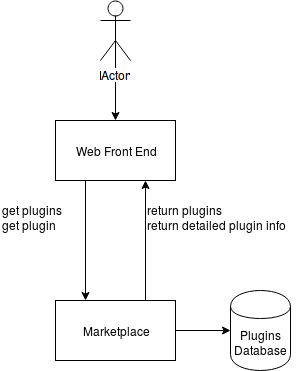
\includegraphics[width=0.5\textwidth]{img/MarketplaceArchitecture.png}
		\end{figure}

	\section{Tables}
		As mentioned before, the most important table in the database is the \textbf{Plugins} table, whose attributes are defined in detail in the following list.

		\begin{itemize}
			\item \emph{id} - A globally unique identification string which can be used to reference this plugin.
			\item \emph{name} - The name of the plugin, as it will appear in lists when users wish to browse the list of plugins.
			\item \emph{author\_id} - The unique authenticated id of the user who uploaded the plugin.
			\item \emph{created\_date} - The date on which the plugin was first uploaded.
			\item \emph{last\_edited\_date} - The date of the most recent update to the plugin.
			\item \emph{version} - A string of numbers representing the current version of the plugin. This is up to the author's discretion.
			\item \emph{description\_short} - A short and concise description, less than 100 characters, which can be displayed in menus to give users a hint as to what the plugin does.
			\item \emph{description\_long} - A much more detailed description of the plugin, which provides detailed instructions for use of the plugin, or other relevant details that the author thinks the users should know.
			\item \emph{up\_goats} - Up-Goats represent the number of users who cast a positive vote for the plugin, meaning that they believe it is valuable and useful.
			\item \emph{down\_goats} - Down-Goats are the opposite of Up-Goats, and count the number of users who voted negatively for the plugin.
		\end{itemize}

		Additionally, some other tables are needed to provide auxiliary information to make the user experience more enjoyable. These are defined below.

		The \textbf{Tags} table holds many tags, which are can be applied to many plugins to group them into related categories.

		\begin{itemize}
			\item \emph{name} - A unique string which represents a tag, which can be applied to a plugin to give it some extra meaning.
			\item \emph{description} - A short description of the tag, or an embellishment of its meaning.
		\end{itemize}

		In order to manifest the \emph{many-to-many} relationship between tags and plugins, a third table, \textbf{PluginTags}, is needed to pair the two together.

		\begin{itemize}
			\item \emph{plugin\_id} - The global id of the plugin paired with a tag.
			\item \emph{tag\_name} - The unique name of a tag which is paired to the above plugin.
		\end{itemize}

		Further, because each plugin records the number of votes for it, and each vote is tied to a specific authenticated user, a table is needed to record this information. The \textbf{UserVotes} table is described below.

		\begin{itemize}
			\item \emph{user\_id} - The unique id of a user.
			\item \emph{plugin\_id} - The unique id of a plugin for which a user has voted.
			\item \emph{vote} - Either 1 or -1, depending on if the vote is an \emph{up\_goat} or \emph{down\_goat}.
		\end{itemize}

		\begin{figure}
			\caption{The tables can be visualized as the schema shown here.}
			\centering
			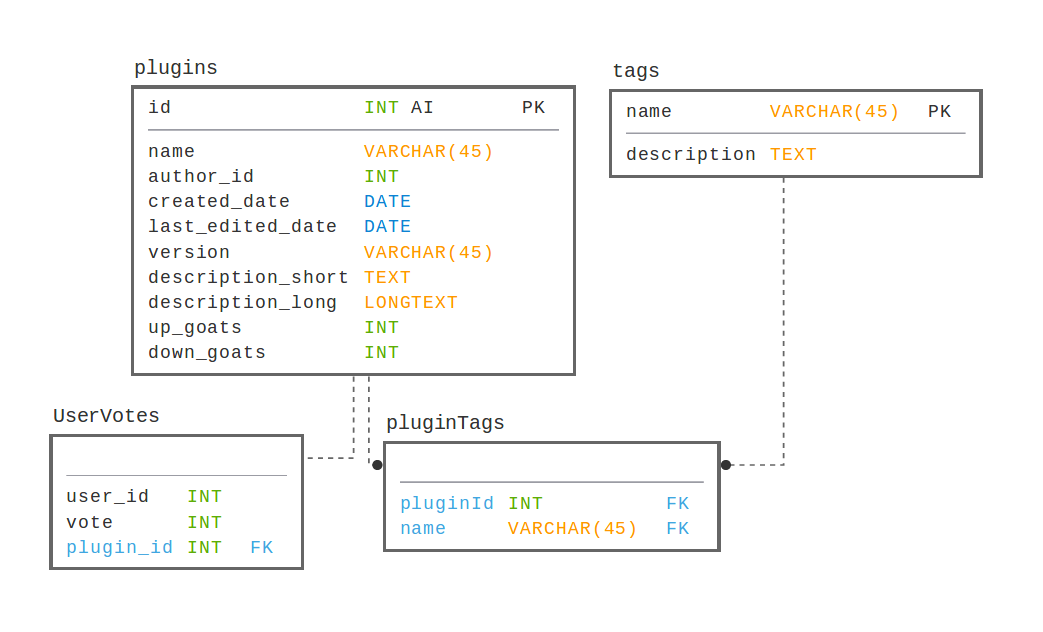
\includegraphics[width=0.8\textwidth]{img/database_schema.png}
		\end{figure}

	\section{File Storage}
		Because the core of each plugin is a collection of files, these will need to be stored in or alongside the database. In order to keep the files synchronized with the contents of the actual relational database, a \textbf{plugins} folder will contain many \verb|.zip| files, each named according the the globally unique id number of the plugin they represent.

\part{REST API}
	This section contains the API documentation for the HTTP methods used to interact with the server, and defines the syntax for making requests, as well as what responses should be expected when requests are made, valid or not.

	\section{GET plugins}
		Returns some basic information about all available plugins, while omitting more specific information like \emph{description\_long}. Some options can be specified to customize the response content, and it is highly encouraged to make use of these, so as to avoid stressing the server by requesting almost the entire contents of the database.

		\subsection{Syntax}
			\verb|GET <URL>/plugins|

			To constrain the results, it is possible to specify some options via a JSON object, such as the example below.

			\lstinputlisting[language=json]{code/get_plugins_options.json}

			More specifically, a \textbf{count} can limit the query to some number of plugins. \textbf{tags} is used to filter the query to only contain plugins whose tags contain all those listed inside that list. \textbf{title\_contains} will filter plugins so that only those whose title contains the supplied text will be returned. \textbf{author\_id} can be used to only return plugins by a specified author.

			It is also possible to request that the returned data be sorted, and this can be done with the \textbf{sort} key, where the \textbf{by} keyword specifies which data category to sort by. The categories are simply any attributes listed in the \textbf{Plugins} table above. Additionally, \textbf{order} can be specified to sort the data either ascendingly or descendingly. When this is omitted, data is sorted ascendingly by default.

		\subsection{Responses}
			\subsubsection{Success}
				In the likely event that the server can retrieve the list of plugins, it will return a \verb|JSON| object containing all the plugins' metadata. The structure of that object is defined below.

				\lstinputlisting[language=json]{code/get_plugins_example.json}

			\subsubsection{Server Error}
				Because no parameters are required, any error, given a proper \verb|URL|, is the fault of the server, and as such, a \verb|500 Internal Error| message will be returned.

	\section{GET a plugin's metadata}
		Returns more detailed information about a specific plugin, including the \emph{description\_long}.

		\subsection{Syntax}
			\verb|GET <URL>/plugin/<PLUGIN_ID>|; \footnotesize{Where \verb|PLUGIN_ID| is the unique id of the plugin.}

		\subsection{Responses}
			\subsubsection{Success}
				If the server successfully finds a plugin with the id specified in the URL, then it will return a JSON object with the structure shown below.

				\lstinputlisting[language=json]{code/get_plugin_example.json}

			\subsubsection{Plugin Not Found}
				If the id specified in the URL does not refer to any existing plugin, then a \verb|404 Not Found| error message will be returned.

			\subsubsection{Server Error}
				If the server fails to retrieve information for a plugin which may or may not exist, or if the server fails in some other way, on its own fault, it will return \verb|500 Internal Error|.

	\section{GET a plugin's zipped files}
		Returns the \verb|.zip| file associated with a plugin whose id is specified in the request.

		\subsection{Syntax}
			\verb|GET <URL>/plugin/<PLUGIN_ID>/files|; \footnotesize{Where \verb|PLUGIN_ID| is the unique id of the plugin.}

		\subsection{Responses}
			\subsubsection{Success}
				If the plugin specified by the given id exists, then the server will return a response consisting of a \verb|200 Ok|, along with header \verb|Content-Type: application/zip|, which specifies that the server has sent a \verb|.zip| file in the response.

			\subsubsection{Plugin Not Found}
				If the id specified in the URL does not refer to any existing plugin, then a \verb|404 Not Found| error message will be returned.

			\subsubsection{Server Error}
				In the event of a server error, despite a possibly valid request, \verb|500 Internal Error| will be returned.

	\section{POST a new plugin}
		To create a new plugin, one must send a POST request with the necessary data.

		\subsection{Syntax}
			\verb|POST <URL>/plugin|; \footnotesize{Where the header \verb|Content-Type| is set to \verb|application/json|, and the content of the POST contains data with the same structure as shown below.}

			\lstinputlisting[language=json]{code/post_plugin_example.json}

		\subsection{Responses}
			\subsubsection{Success}
				If the server is able to successfully create the plugin without any constraint conflicts or other issues, a \verb|201 Created| message will be returned, as well as the id of the newly created plugin in a json object as shown below. Once the plugin has been created, one must then use a PUT request to upload the zipped plugin files to the server, using the received id.

				\lstinputlisting[language=json]{code/post_plugin_success_response.json}

				Note that after some time, if a created plugin has not had some files added to it, that plugin will be removed automatically. Therefore, the files should be uploaded immediately after the success of this request is returned.

			\subsubsection{Constraint Violation}
				Due to the nature of entering data into a database, certain values must not be null, certain values must be unique, etc. If the content of the POST request does not satisfy the constraints set forth for the database, the server will return \verb|400 Bad Request|.

			\subsubsection{Authorization Error}
				If the sender of the request is not authorized via Auth0, then the server will return \verb|401 Unauthorized|, as it is necessary for a user to be logged in to create a plugin so it can be traced to that user.

			\subsubsection{Server Error}
				If for some reason the server encounters an error beyond what was defined above, it will return \verb|500 Internal Error|.

	\section{PUT .zip file to a plugin}
		Immediately after creating a plugin, one should use this request to upload a \verb|.zip| file to the server, with the same authenticated user as the author of the plugin. Nobody else will be allowed to upload to the plugin except for the author.

		This method is also used to update the files of an existing plugin, which will overwrite any existing files.

		\subsection{Syntax}
			\verb|PUT <URL>/plugin/<PLUGIN_ID>/files|; \footnotesize{Where \verb|PLUGIN_ID| is the unique id of the plugin.}

			The content of the request contains the \verb|.zip| file, which itself contains the contents of the plugin.

		\subsection{Responses}
			\subsubsection{Success}
				If the server is able to successfully receive the zipped files and store it, the server will return \verb|200 Ok|.

			\subsubsection{Authorization Error}
				If the sender of the request is not authorized via Auth0, and the author of the plugin to which they are attempting to upload the files, a \verb|401 Unauthorized| error will be returned.

			\subsubsection{No Files}
				Because the whole point of this request is to upload a \verb|.zip| file, if none is provided, the server will return a \verb|400 Bad Request| error.

			\subsubsection{Plugin Not Found}
				If the id provided does not refer to any existing plugin, then \verb|404 Not Found| will be returned.

			\subsubsection{Server Error}
				Beyond all the possible user errors written above, if the server fails on its own accord, then it will return a \verb|500 Internal Error|, at which point the user can assume that their files have not been saved on the server.

	\section{DELETE a plugin}
		This will irreversibly delete both a plugin and any zipped files associated with it. This action must be performed by either an administrator or the plugin owner.

		\subsection{Syntax}
			\verb|DELETE <URL>/plugin/<PLUGIN_ID>|; \footnotesize{Where \verb|PLUGIN_ID| is the unique id of the plugin.}

		\subsection{Responses}
			\subsubsection{Success}
				If the resource is deleted successfully, as well as the associated files, then the server will return \verb|205 Reset Content|, as it will be necessary for the user to refresh their content view now that the plugin has been deleted.

			\subsubsection{Authorization Error}
				If the user is not both authenticated, and the author of the plugin, then they are forbidden from deleting the plugin. The server will return \verb|401 Unauthorized|.

			\subsubsection{Plugin Not Found}
				If the id provided does not refer to any existing plugin, then \verb|404 Not Found| will be returned.

			\subsubsection{Server Error}
				If for some reason, the server is not able to delete both the plugin in the database and the associated files, then it will return \verb|500 Internal Error|.

	\section{PATCH a plugin's metadata}
		Using this method, it is possible to update parts of the plugin's metadata, if the user is authenticated as the author of the plugin.

		\subsection{Syntax}
			\verb|PATCH <URL>/plugin/<PLUGIN_ID>|; \footnotesize{Where \verb|PLUGIN_ID| is the unique id of the plugin.}

			The new data can be sent in the same format as when POSTing a new plugin, although here it is permissable to omit fields which do not need to be updated. Therefore, the following example from the POST request is applicable here too.

			\lstinputlisting[language=json]{code/post_plugin_example.json}

		\subsection{Responses}
			\subsubsection{Success}
				If the server can successfully use the data which is sent to update the plugin's metadata, then the server will return a \verb|205 Reset Content| code, as the user's view should be updated to reflect the successful changes.

			\subsubsection{Authorization Error}
				If the user is not both authenticated, and the author of the plugin, then they are forbidden from updating the metadata of the plugin. The server will therefore return \verb|401 Unauthorized|.

			\subsubsection{Plugin Not Found}
				If the id provided does not refer to any existing plugin, then \verb|404 Not Found| will be returned.

			\subsubsection{Server Error}
				If for some reason, the server is not able to update the metadata and fails internally, it will return a \verb|500 Internal Error|.

	\section{POST to vote for a plugin}
		Use this method to allow a user to cast a vote for a particular plugin. The vote will be traced to their authenticated user id, so that the vote can be changed at any time simply by calling this method again.

		\subsection{Syntax}
			\verb|POST <URL>/plugin/<PLUGIN_ID>/vote|; \footnotesize{Where \verb|PLUGIN_ID| is the unique id of the plugin.}

			The content of the post request must then follow the structure shown below.

			\lstinputlisting[language=json]{code/vote_example.json}

			Note that the value of the key \verb|"vote"| may be either 1 (\emph{up\_goat}), 0 (\emph{reset vote}), or -1 (\emph{down\_goat}). Whatever value is sent will override any previous vote by that user.

		\subsection{Responses}
			\subsubsection{Success}
				If the user's vote is successfully cast, then the server will return \verb|205 Reset Content|, indicating that the user's document should reflect the change in vote.

			\subsubsection{Authorization Error}
				Because only authorized users are allowed to vote, those who are not will receive a \verb|401 Unauthorized| response when attempting to send this request.

			\subsubsection{Plugin Not Found}
				If the id provided does not refer to any existing plugin, then \verb|404 Not Found| is returned.

			\subsubsection{Server Error}
				If it is not possible for the server to register the vote, then it will return \verb|500 Internal Error|, and the user should interpret this as that no change has been made to the votes.

\end{document}